\documentclass[11pt, a4paper]{article}

% --- Preamble ---
\usepackage[utf8]{inputenc} % Allows inputting UTF-8 characters
\usepackage[T1]{fontenc}    % Optimizes font encoding
\usepackage[english]{babel} % Language settings
\usepackage[margin=1in]{geometry} % Page margins
\usepackage{amsmath, amssymb} % For mathematical symbols and equations
\usepackage{graphicx}       % For including images
\graphicspath{{media/}}     % Tells LaTeX where to look for images
\usepackage{hyperref}       % For clickable links in the PDF (e.g., table of contents)
\hypersetup{
    colorlinks=true,
    linkcolor=blue,
    filecolor=magenta,
    urlcolor=cyan,
    pdftitle={Discrete Mathematics Project Report: Graph Theory and Graph Coloring},
    pdfauthor={Your Name},
    pdfsubject={Graph Theory, Graph Coloring, Discrete Mathematics},
    pdfkeywords={Graph, Coloring, Chromatic Number, Applications},
}
\usepackage{fancyhdr}       % For custom headers/footers
\usepackage{enumitem}       % For customizing list environments
\usepackage{setspace}       % For setting line spacing

% Custom header/footer setup
\pagestyle{fancy}
\fancyhf{} % Clear all headers/footers
\fancyhead[L]{Discrete Maths Project}
\fancyhead[R]{Graph Theory & Coloring}
\fancyfoot[C]{\thepage}
\renewcommand{\headrulewidth}{0.4pt}
\renewcommand{\footrulewidth}{0.4pt}

% Line spacing
\onehalfspacing % 1.5 line spacing

% --- Title Page Information ---
\title{\textbf{Project Report on Graph Theory and Graph Coloring}}
\author{
    \textbf{Your Name} \\
    Student ID: \texttt{XXXXXXXX} \\
    Department of \textit{Your Department} \\
    \textit{Your University}
}
\date{\today} % Or specify a date like \date{October 26, 2023}

% --- Document Start ---
\begin{document}

\maketitle % Displays the title page

\thispagestyle{empty} % No page number on the title page
\newpage

% --- Abstract ---
\begin{abstract}
This report delves into the fascinating world of Graph Theory, a fundamental area of Discrete Mathematics, with a particular focus on Graph Coloring. We begin by introducing the basic definitions and concepts of graphs, including vertices, edges, and various types of graphs. Following this, the core principles of graph coloring are explored, defining concepts such as chromatic number and discussing common algorithms like the greedy coloring algorithm. The report highlights diverse applications of graph coloring in real-world scenarios, ranging from scheduling and resource allocation to map coloring and register allocation in compilers. Finally, a conclusion summarizes the key findings and emphasizes the pervasive importance of graph theory and its coloring techniques in solving complex problems across different disciplines.
\end{abstract}

\newpage
\tableofcontents % Generates the table of contents
\newpage

% --- Introduction ---
\section{Introduction}
Graph Theory, a vibrant branch of discrete mathematics, provides a powerful framework for modeling and analyzing relationships between objects. It consists of a set of vertices (or nodes) and a set of edges (or links) connecting pairs of these vertices. Originating from Euler's solution to the Königsberg Bridge Problem in 1736, graph theory has evolved into an indispensable tool across numerous fields, including computer science, engineering, operations research, biology, and social sciences.

This report aims to provide a comprehensive overview of fundamental graph theory concepts, culminating in a detailed discussion of graph coloring. Graph coloring, a special case of graph labeling, assigns labels (colors) to elements of a graph subject to certain constraints. Its elegance lies in its ability to model complex resource allocation and scheduling problems, making it a cornerstone in algorithmic problem-solving. We will explore the definitions, algorithms, and practical applications of graph coloring, demonstrating its significance in solving real-world challenges.

% --- Fundamentals of Graph Theory ---
\section{Fundamentals of Graph Theory}
A graph $G$ is formally defined as an ordered pair $(V, E)$, where $V$ is a finite, non-empty set of vertices (or nodes) and $E$ is a set of edges (or links) connecting pairs of distinct vertices.

\subsection{Basic Definitions}
\begin{itemize}[noitemsep,topsep=3pt,parsep=3pt,partopsep=0pt]
    \item \textbf{Vertex (Node)}: A fundamental unit of which graphs are formed.
    \item \textbf{Edge (Link)}: A connection between two vertices. An edge $(u,v)$ connects vertex $u$ and vertex $v$.
    \item \textbf{Adjacent Vertices}: Two vertices are adjacent if they are connected by an edge.
    \item \textbf{Degree of a Vertex}: The number of edges incident to a vertex.
    \item \textbf{Path}: A sequence of distinct vertices such that consecutive vertices are adjacent.
    \item \textbf{Cycle}: A path that starts and ends at the same vertex.
\end{itemize}

\subsection{Types of Graphs}
\begin{itemize}[noitemsep,topsep=3pt,parsep=3pt,partopsep=0pt]
    \item \textbf{Undirected Graph}: Edges have no direction. If $(u,v)$ is an edge, then $(v,u)$ is also an edge.
    \item \textbf{Directed Graph (Digraph)}: Edges have a direction, usually indicated by an arrow. If $(u,v)$ is an edge, it means there's a connection from $u$ to $v$, but not necessarily from $v$ to $u$.
    \item \textbf{Weighted Graph}: Each edge has an associated numerical value (weight), often representing cost, distance, or capacity.
    \item \textbf{Complete Graph ($K_n$)}: A graph where every pair of distinct vertices is connected by a unique edge.
    \item \textbf{Tree}: A connected undirected graph with no simple cycles.
\end{itemize}

% Example of an image inclusion (from your media folder)
\begin{figure}[h!]
    \centering
    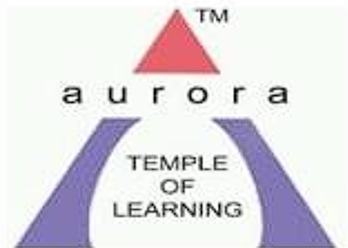
\includegraphics[width=0.6\textwidth]{aurora_logo.png}
    \caption{Example image: Aurora Logo}
    \label{fig:aurora_logo}
\end{figure}

\section{Graph Coloring}
Graph coloring is an assignment of labels (colors) to the elements of a graph subject to certain constraints. Most commonly, it refers to \textit{vertex coloring}.

\subsection{Vertex Coloring}
Vertex coloring is a way of coloring the vertices of a graph such that no two adjacent vertices share the same color. The goal is often to use the minimum number of colors possible.

\begin{itemize}[noitemsep,topsep=3pt,parsep=3pt,partopsep=0pt]
    \item \textbf{Proper Coloring}: A coloring where no two adjacent vertices have the same color.
    \item \textbf{Chromatic Number ($\chi(G)$)}: The minimum number of colors required for a proper coloring of a graph $G$.
\end{itemize}

For example, a complete graph $K_n$ requires $n$ colors, since every vertex is adjacent to every other vertex. Therefore, $\chi(K_n) = n$.

\subsection{Algorithms for Graph Coloring}
Finding the chromatic number of a graph is an NP-hard problem, meaning there's no known polynomial-time algorithm for it. However, several heuristic and approximation algorithms exist for finding a coloring.

\subsubsection{Greedy Coloring Algorithm}
The greedy coloring algorithm is a simple heuristic approach. It works as follows:
\begin{enumerate}[noitemsep,topsep=3pt,parsep=3pt,partopsep=0pt]
    \item Order the vertices of the graph (e.g., arbitrarily, or by degree).
    \item Assign the first vertex the first available color (e.g., color 1).
    \item For each subsequent vertex, assign it the smallest available color that has not been used by any of its already-colored neighbors.
\end{enumerate}
While easy to implement, greedy coloring does not always yield an optimal coloring (i.e., it might use more colors than the chromatic number).

\subsubsection{Welsh-Powell Algorithm}
A specific variant of greedy coloring that often performs better. Vertices are ordered in decreasing order of their degrees. The greedy coloring procedure is then applied to this ordered list.

\subsection{Applications of Graph Coloring}
Graph coloring has numerous practical applications:

\begin{enumerate}[noitemsep,topsep=3pt,parsep=3pt,partopsep=0pt]
    \item \textbf{Timetabling and Scheduling}: Assigning courses to time slots such that no two courses requiring the same resource (e.g., lecturer, classroom) are scheduled simultaneously. Vertices represent courses, edges represent conflicts, and colors represent time slots.
    \item \textbf{Register Allocation (Compilers)}: In computer science, compilers use graph coloring to allocate CPU registers to program variables. Variables that are simultaneously "live" (in use) cannot be assigned the same register. Vertices are variables, edges connect simultaneously live variables, and colors are registers.
    \item \textbf{Map Coloring}: The classic "Four Color Theorem" states that any planar map can be colored with at most four colors such that no two adjacent regions have the same color. Vertices are regions, edges connect adjacent regions, and colors are actual colors for the map.
    \item \textbf{Frequency Assignment}: Assigning frequencies to radio stations or mobile phone towers to avoid interference. Vertices are transmitters, edges represent interference, and colors are frequencies.
    \item \textbf{Sudoku Puzzle}: A Sudoku grid can be modeled as a graph coloring problem.
\end{enumerate}

% Another example of an image (from your media folder)
\begin{figure}[h!]
    \centering
    
\includegraphics[width=0.7\textwidth]{header.png}
    \caption{Another example image: Header Graphic}
    \label{fig:header_graphic}
\end{figure}

\section{Conclusion}
Graph Theory provides a versatile mathematical language for describing complex systems and relationships. From its humble beginnings with Euler's work, it has grown into an expansive field with profound implications for modern technology and science. Graph coloring, a core concept within this field, exemplifies how abstract mathematical ideas can be leveraged to solve tangible problems.

The ability to efficiently color graphs, even with the inherent computational challenges, directly impacts various real-world applications, from optimizing resource allocation in computing to resolving conflicts in scheduling. While finding optimal colorings remains a hard problem, the development of heuristic algorithms and the continuous search for better solutions highlight the ongoing relevance and research interest in this area. Understanding graph theory and graph coloring is thus essential for anyone venturing into fields requiring sophisticated problem-solving and systems analysis.

\newpage
% --- Bibliography ---
\begin{thebibliography}{99} % The 99 specifies the width of the label
    \bibitem{Diestel2017}
    R. Diestel. \textit{Graph Theory}. 5th ed., Graduate Texts in Mathematics, vol. 173. Springer, 2017.

    \bibitem{Rosen2018}
    K. H. Rosen. \textit{Discrete Mathematics and Its Applications}. 8th ed., McGraw-Hill Education, 2018.

    \bibitem{West2001}
    D. B. West. \textit{Introduction to Graph Theory}. 2nd ed., Prentice Hall, 2001.

    \bibitem{wikipedia_graph_coloring}
    Wikipedia contributors. Graph Coloring. \textit{Wikipedia, The Free Encyclopedia}. \url{https://en.wikipedia.org/wiki/Graph_coloring}. Accessed: \today.
\end{thebibliography}

\end{document}